\documentclass{beamer}

\usepackage[T1]{fontenc}
\usepackage{lmodern}
\usepackage[useregional]{datetime2}
\usepackage{hyphenat}
%\RequirePackage[skip=0.5em,indent=3ex]{parskip}
\usepackage{graphicx,float,quoting,pdfpages}
%\usepackage[hidelinks,colorlinks=true,urlcolor=blue,linkcolor=black]{hyperref}
%\usepackage[all]{hypcap}
\usepackage{polyglossia}
\setdefaultlanguage[variant=brazilian]{portuguese}

\usetheme{metropolis}           % Use metropolis theme

\title{Projeto de divulgação científica --- Química I (CCM0114)}
\subtitle{Produção e consumo sustentáveis}

\date{6 de dezembro, 2020}

\author{Beatriz Brajal \and Isabella Basso \and João Gabriel Borges}

\institute{Universidade de São Paulo --- Ciências Moleculares}


\begin{document}
  \begin{frame}
  	\titlepage % Print the title page as the first slide
  \end{frame}
  
  \begin{frame}{Sumário}
  	\tableofcontents
  \end{frame}
  
  \section{Posts da Beatriz --- Planejamento}
  
  \begin{frame}{Tema}
  	\begin{block}{Produção e consumo responsáveis (PCS)}
  		\begin{itemize}
  			\item Baseado no objetivo de desenvolvimento sustentável 12 (ODS 12) da ONU.
  			\item São 17 objetivos no total.
  		\end{itemize}
  	
  		\bigskip
  	
	  	\begin{quotation}
	  		\itshape ``Assegurar padrões de produção e de consumo sustentáveis.''
	  		\par\raggedleft--- \textup{ONU}, ODS 12 \textup{(enunciado original)}
	  		
	  	\end{quotation}
  	\end{block}
  	
  \end{frame}

	\begin{frame}{Post 1}
		\begin{minipage}{0.49\linewidth}
			\centering
			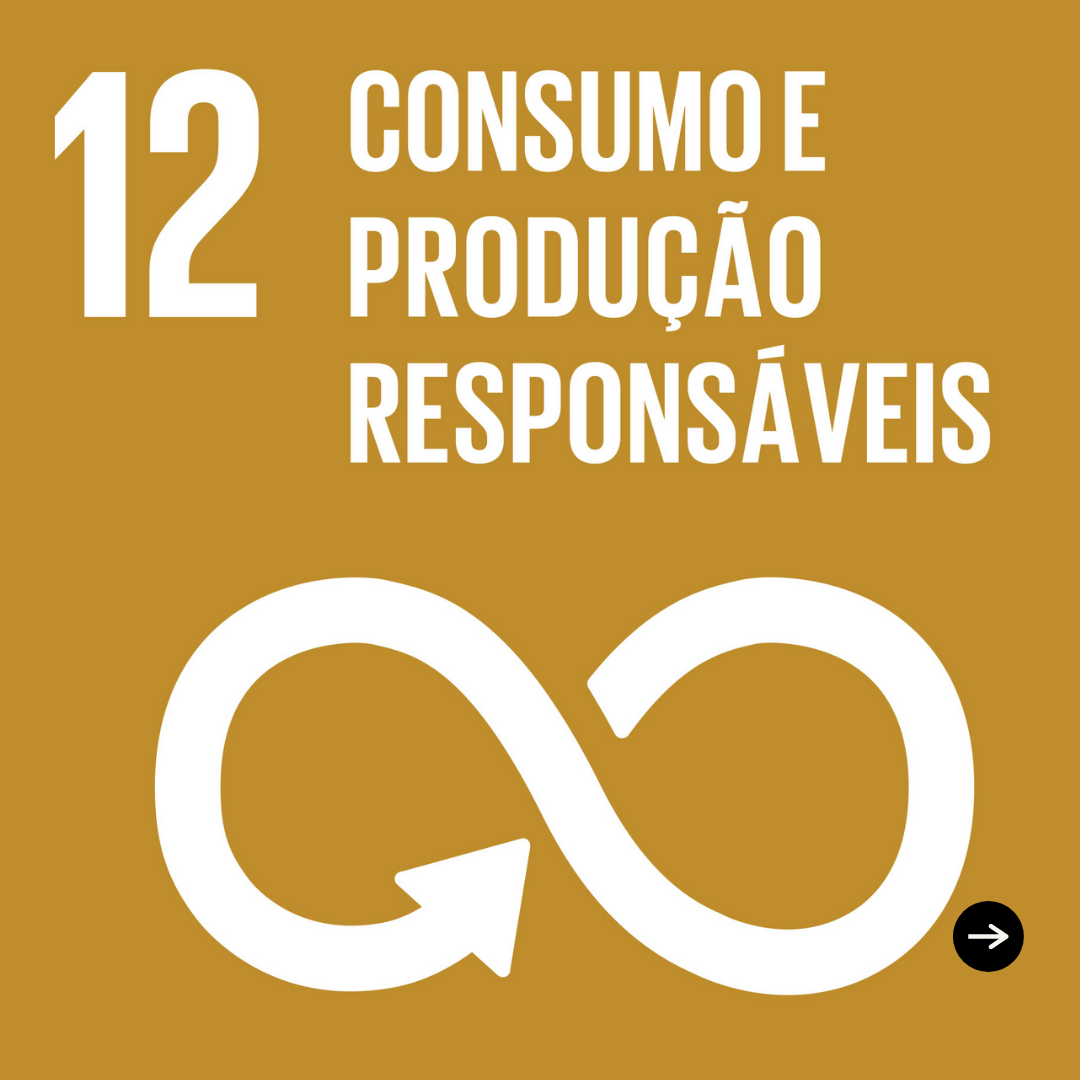
\includegraphics[width=\linewidth]{Post 1/1.png}
		\end{minipage}
		\hfill
		\begin{minipage}{0.49\linewidth}
			\centering
			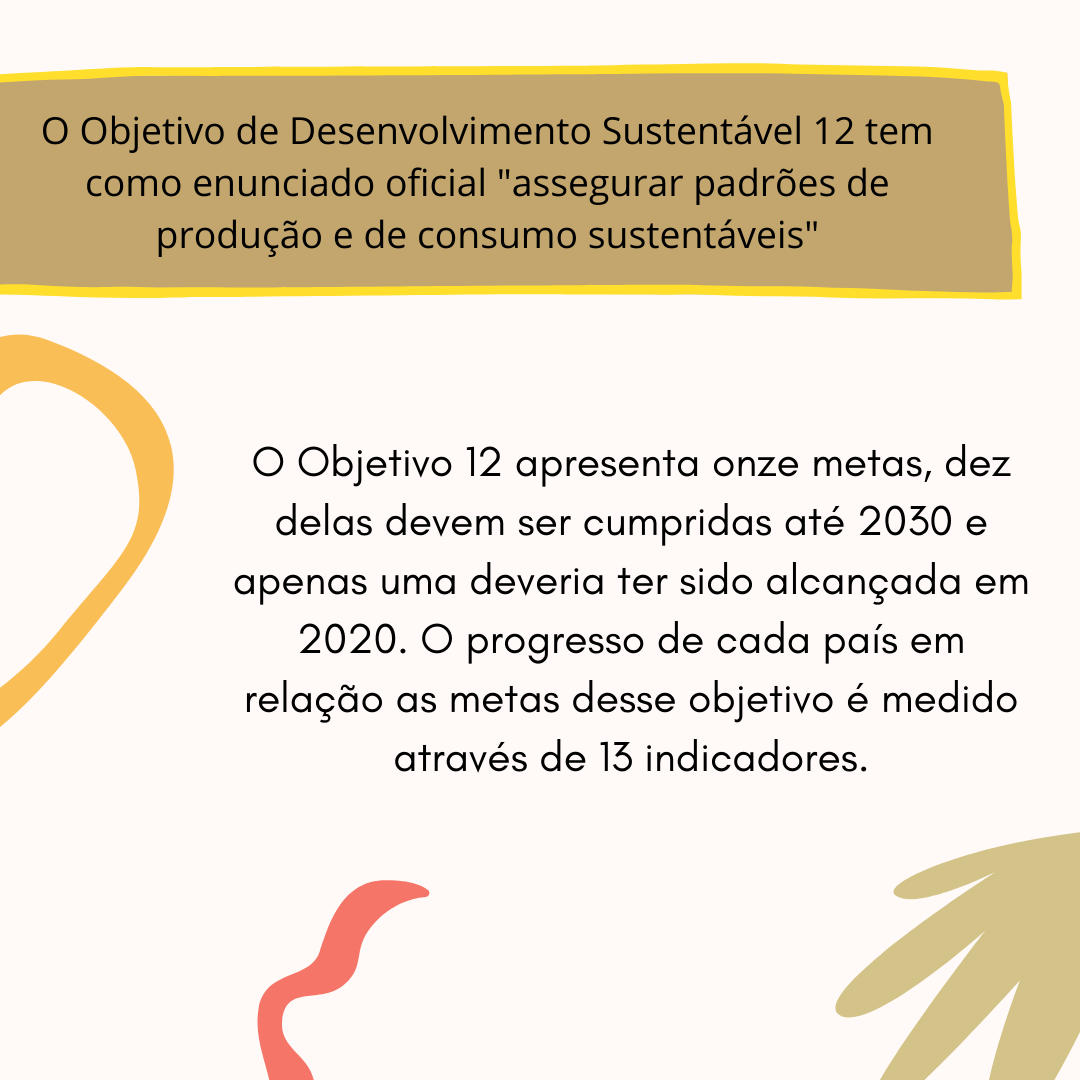
\includegraphics[width=\linewidth]{Post 1/2.png}
		\end{minipage}
	\end{frame}

	\begin{frame}{Post 1}
		\begin{minipage}{0.49\linewidth}
			\centering
			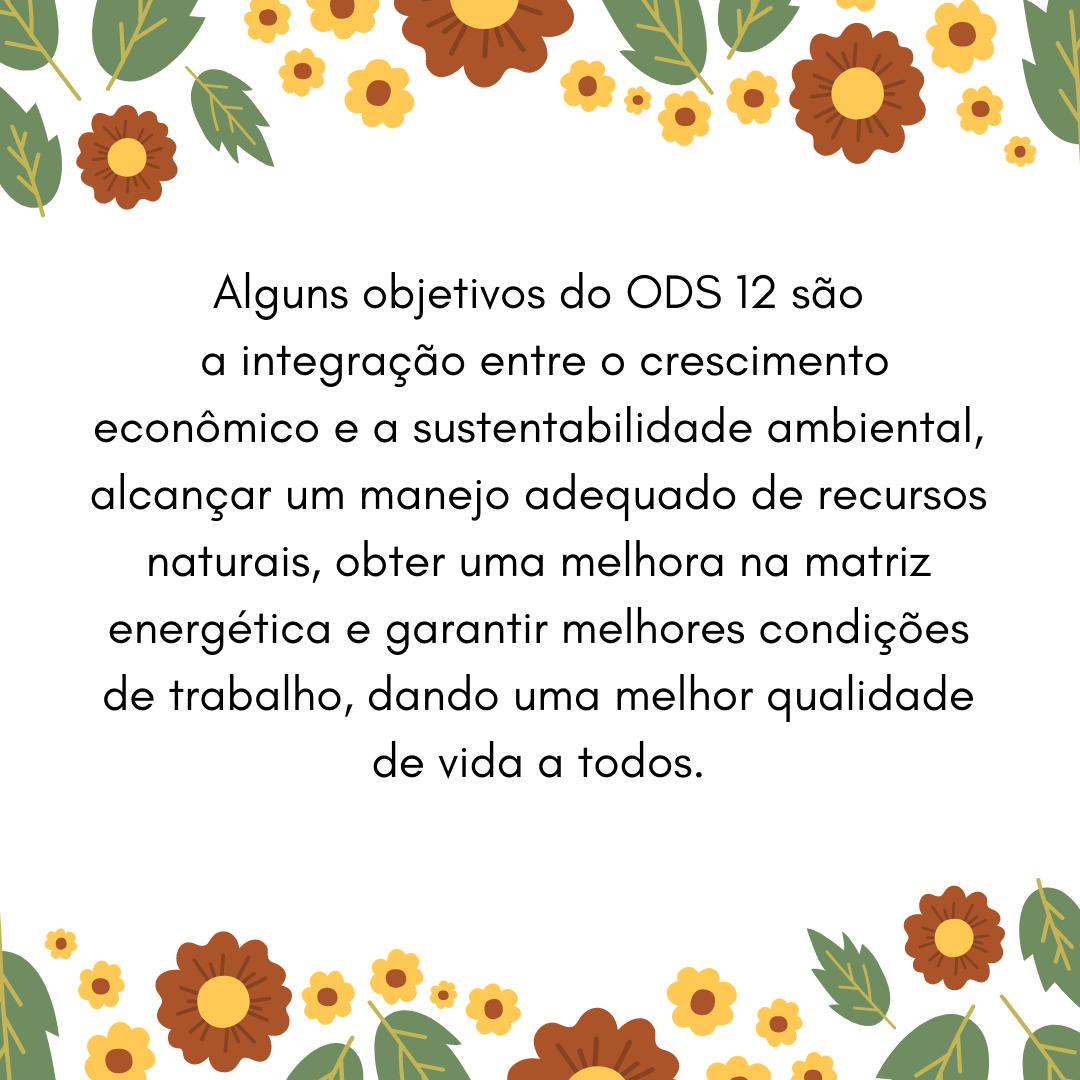
\includegraphics[width=\linewidth]{Post 1/3.png}
		\end{minipage}
		\hfill
		\begin{minipage}{0.49\linewidth}
			\centering
			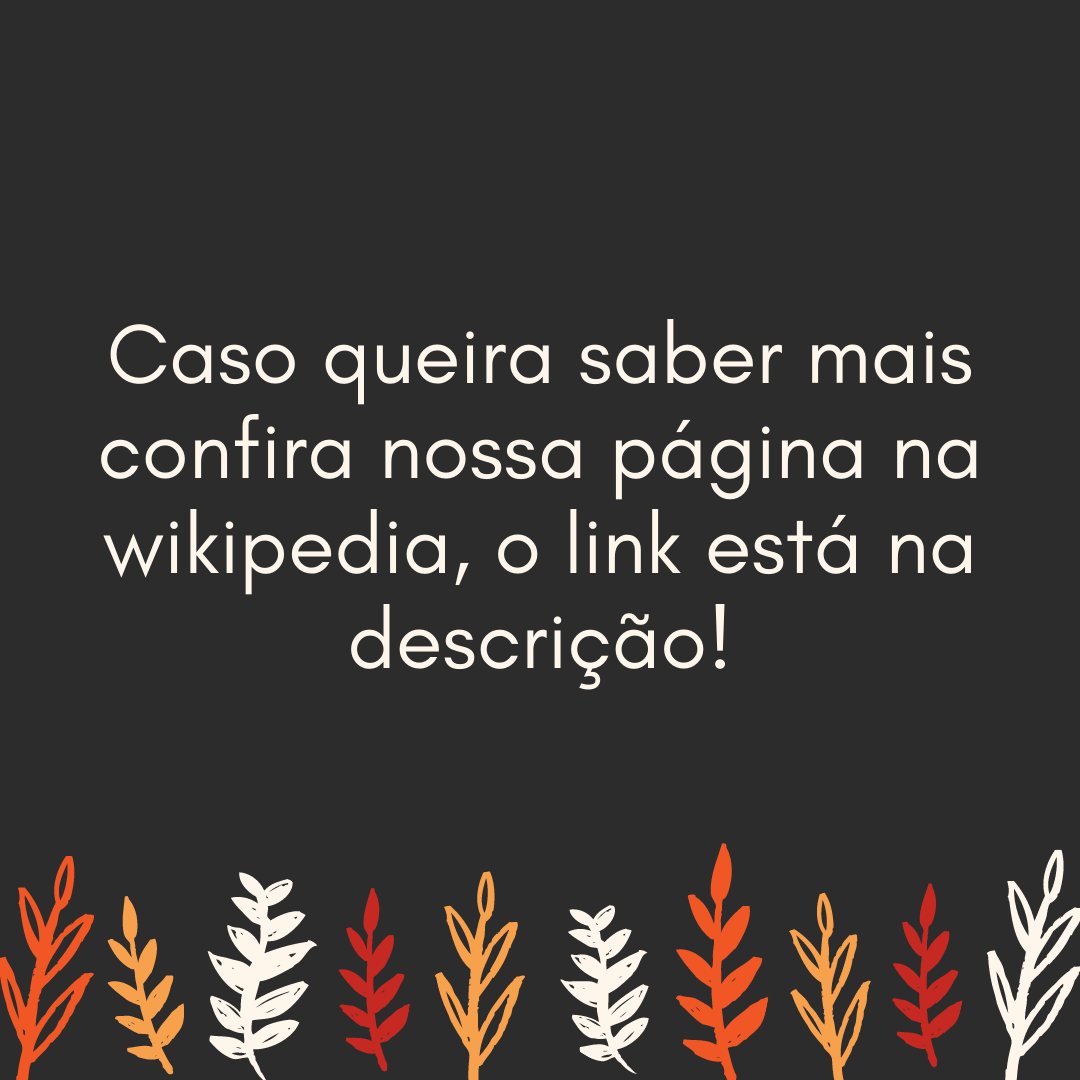
\includegraphics[width=\linewidth]{Post 1/4.png}
		\end{minipage}
	\end{frame}

	\begin{frame}{Post 2}
		\begin{minipage}{0.49\linewidth}
			\centering
			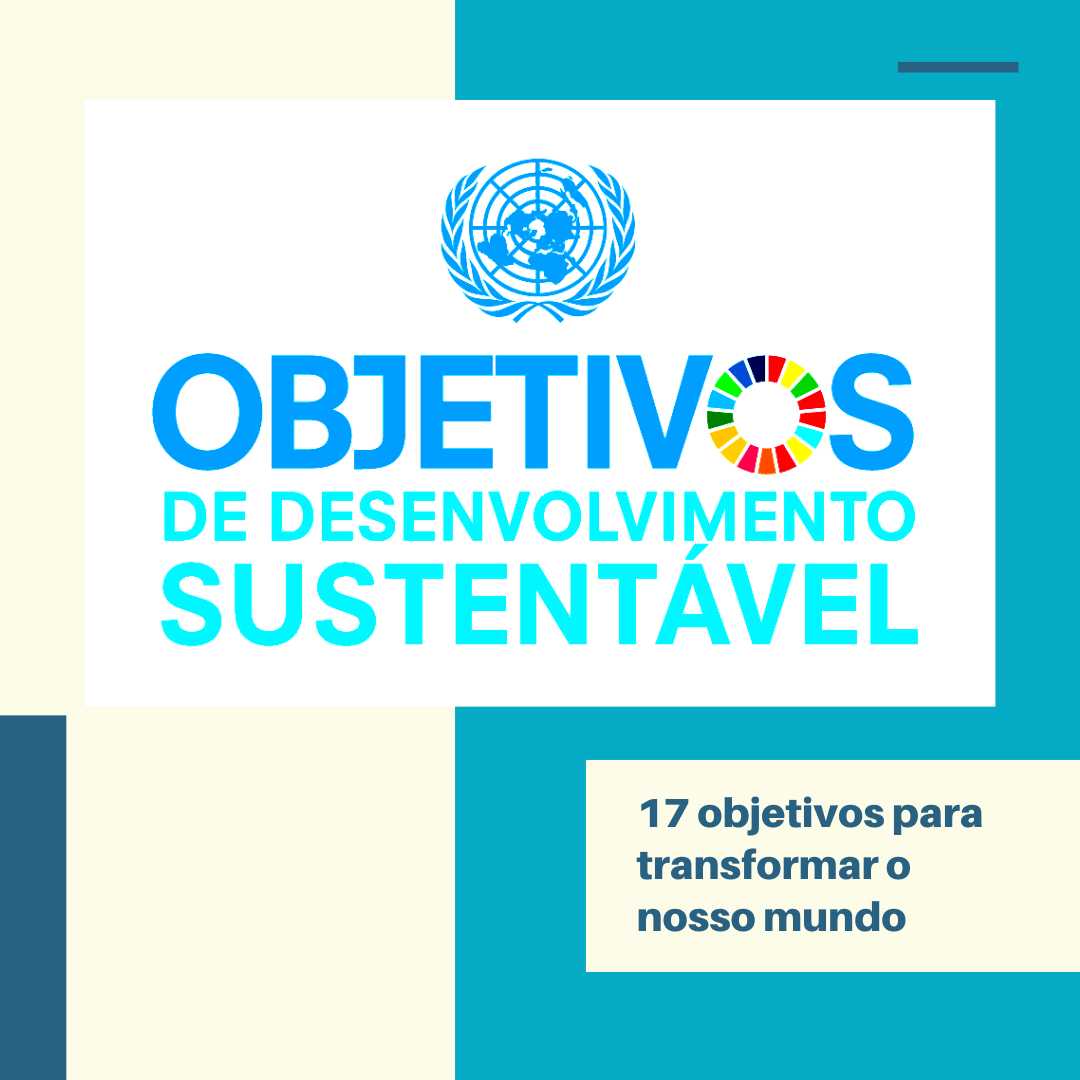
\includegraphics[width=\linewidth]{Post 2/1.png}
		\end{minipage}
		\hfill
		\begin{minipage}{0.49\linewidth}
			\centering
			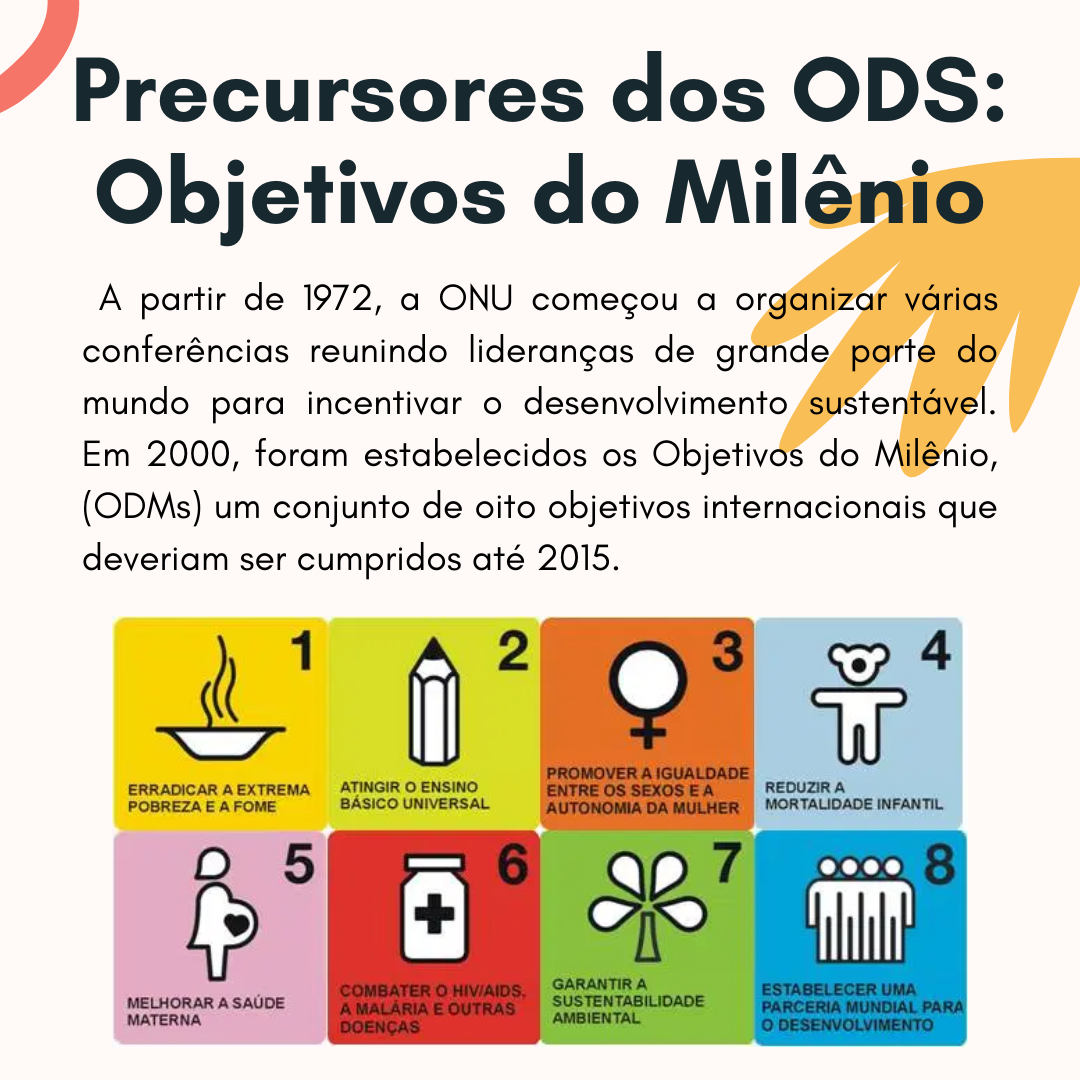
\includegraphics[width=\linewidth]{Post 2/2.png}
		\end{minipage}
	\end{frame}
	
	\begin{frame}{Post 2}
		\begin{minipage}{0.49\linewidth}
			\centering
			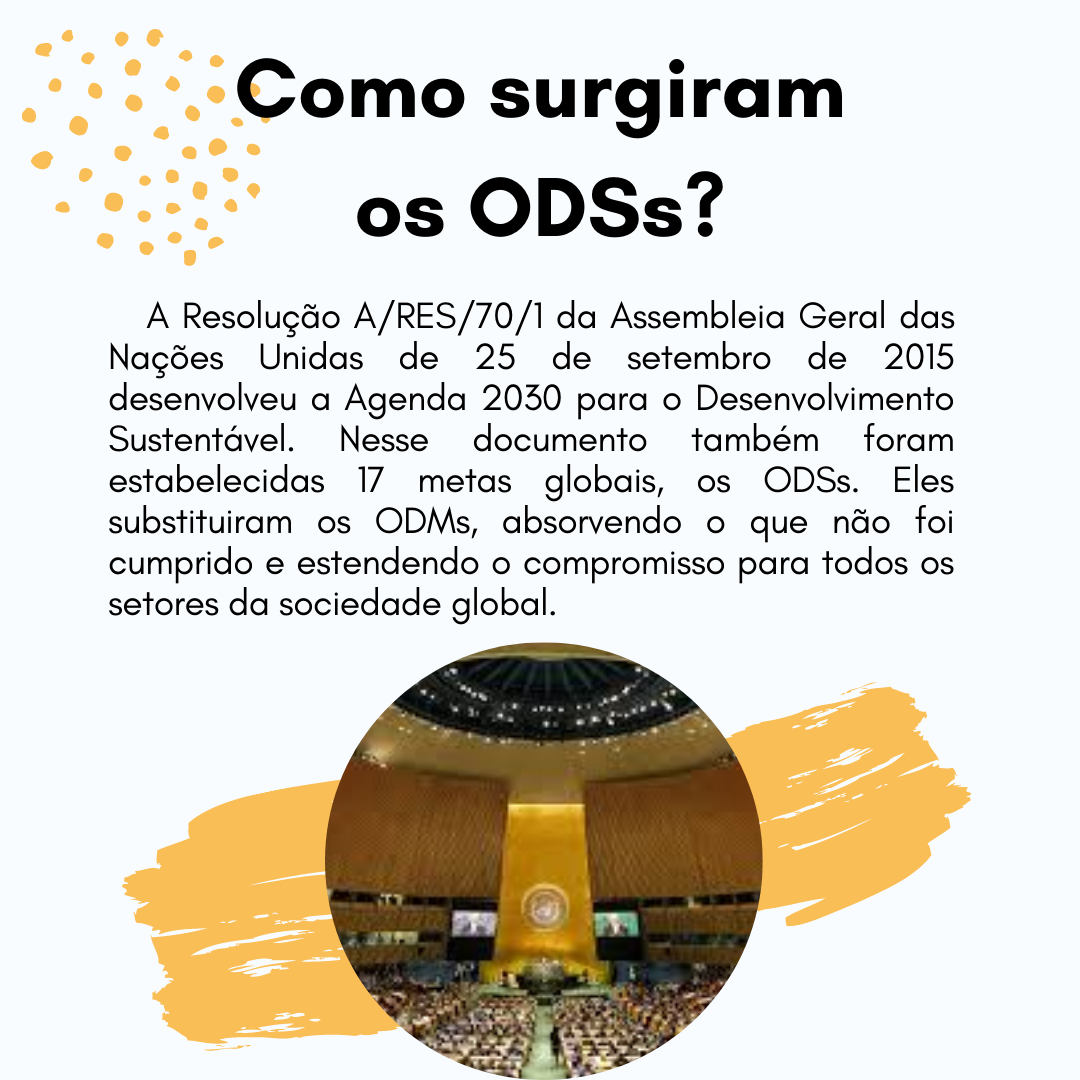
\includegraphics[width=\linewidth]{Post 2/3.png}
		\end{minipage}
		\hfill
		\begin{minipage}{0.49\linewidth}
			\centering
			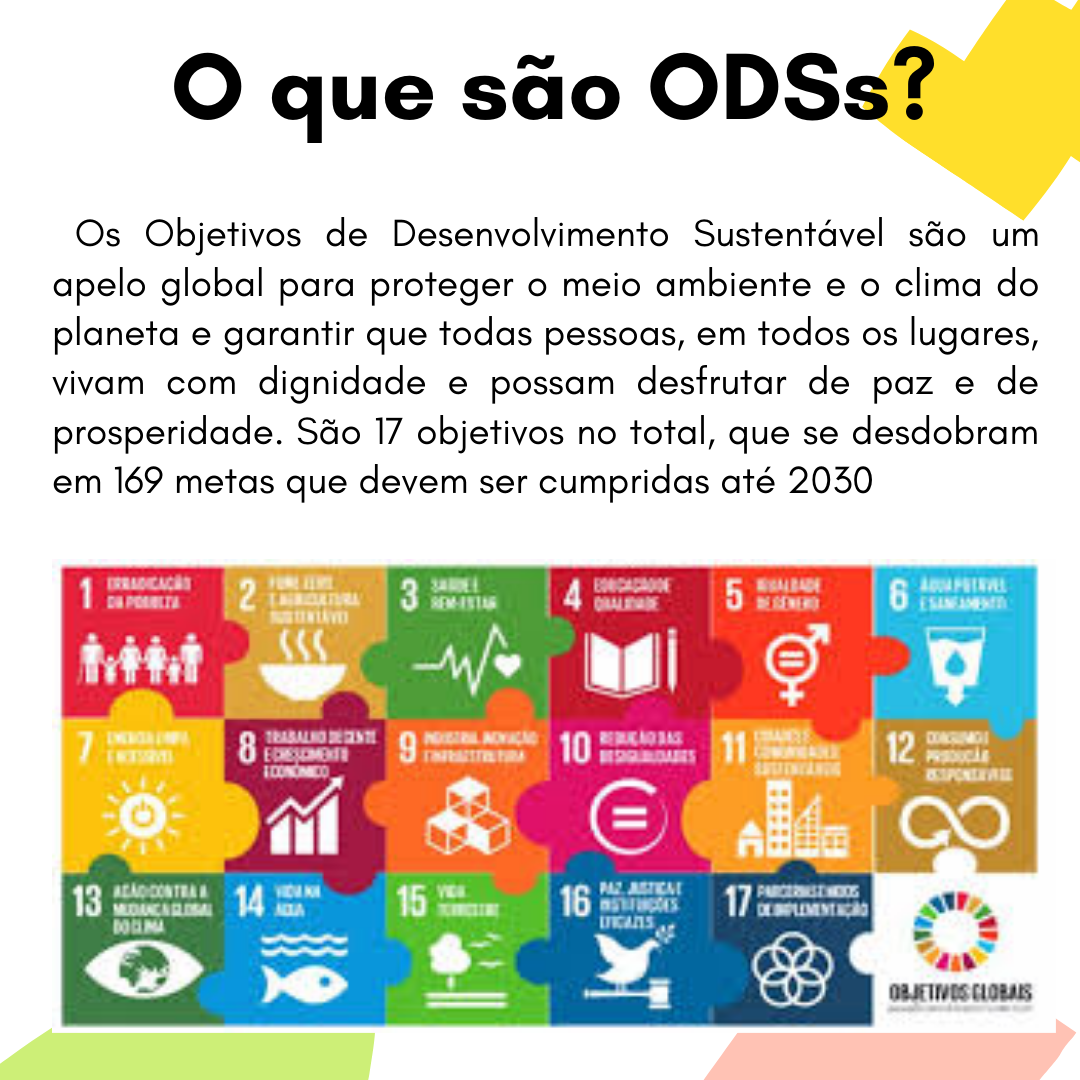
\includegraphics[width=\linewidth]{Post 2/4.png}
		\end{minipage}
	\end{frame}

	\section{Posts do João Gabriel --- Metas da ODS e progresso}

	\begin{frame}[allowframebreaks]{Metas da ODS 12}
		\begin{itemize}
			\item 12.1: Implementar o Plano Decenal de Programas sobre Produção e Consumo Sustentáveis.
			\item 12.2: Gestão sustentável e o uso eficiente dos recursos naturais.
			\item 12.3: Reduzir pela metade o desperdício de alimentos per capita mundial.
			\item 12.4: Gestão responsável de produtos químicos e resíduos.
			\item 12.5: Reduzir substancialmente a geração de resíduos.
			\item 12.6: Incentivar as empresas a adotar práticas sustentáveis e relatórios de sustentabilidade.
			\item 12.7: Promover práticas de compras públicas sustentáveis.
			\item 12.8: Promover a compreensão universal de estilos de vida sustentáveis.
			\item 12.a: Apoiar a capacidade científica e tecnológica dos países em desenvolvimento para consumo e produção sustentáveis.
			\item 12.b: Desenvolver e implementar ferramentas para monitorar o turismo sustentável.
			\item 12.c: Remover distorções de mercado que incentivam o consumo desnecessário.
		\end{itemize}
	\end{frame}

	\begin{frame}{Post 3}
		\begin{minipage}{0.49\linewidth}
			\centering
			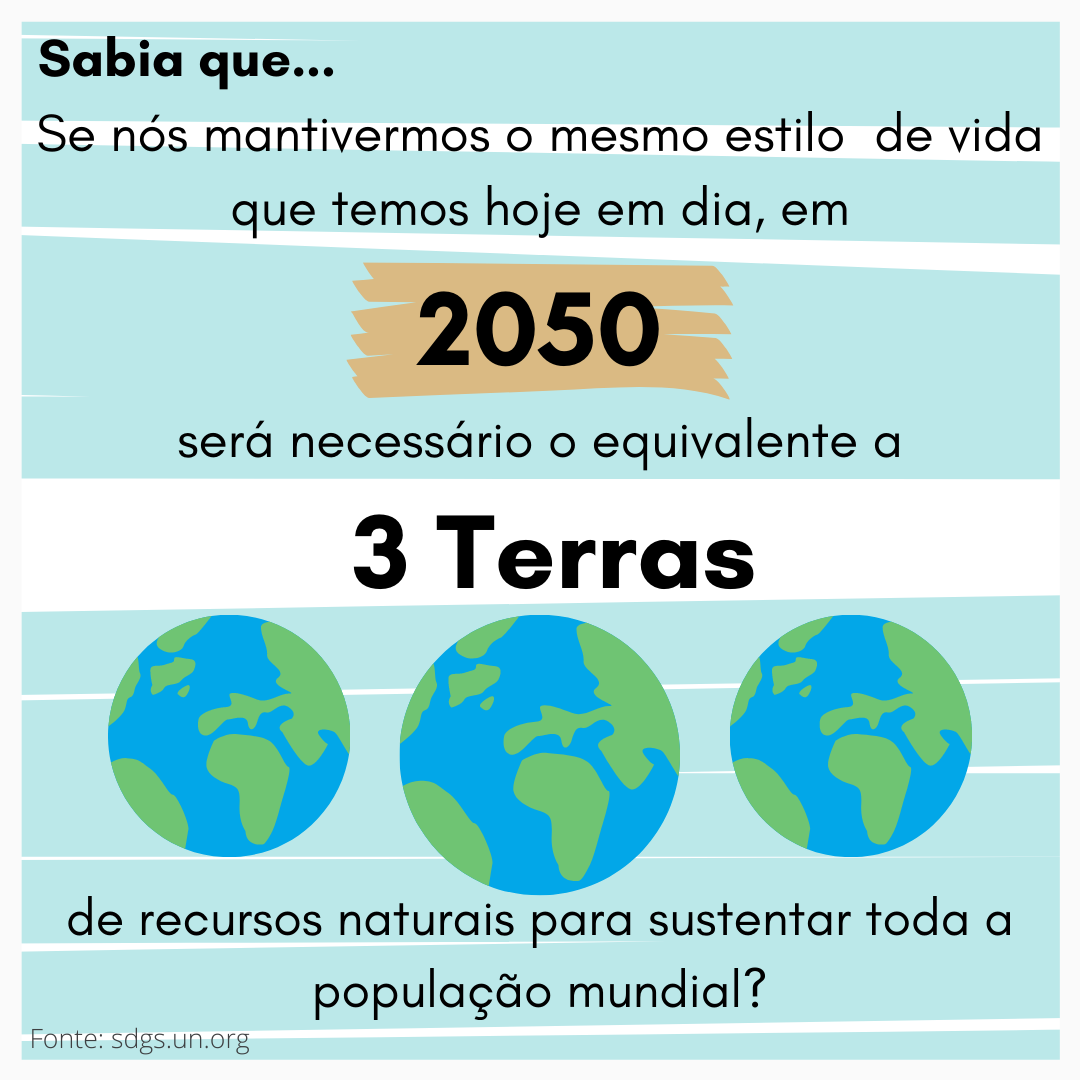
\includegraphics[width=\linewidth]{Post 3/1.png}
		\end{minipage}
		\hfill
		\begin{minipage}{0.49\linewidth}
			\centering
			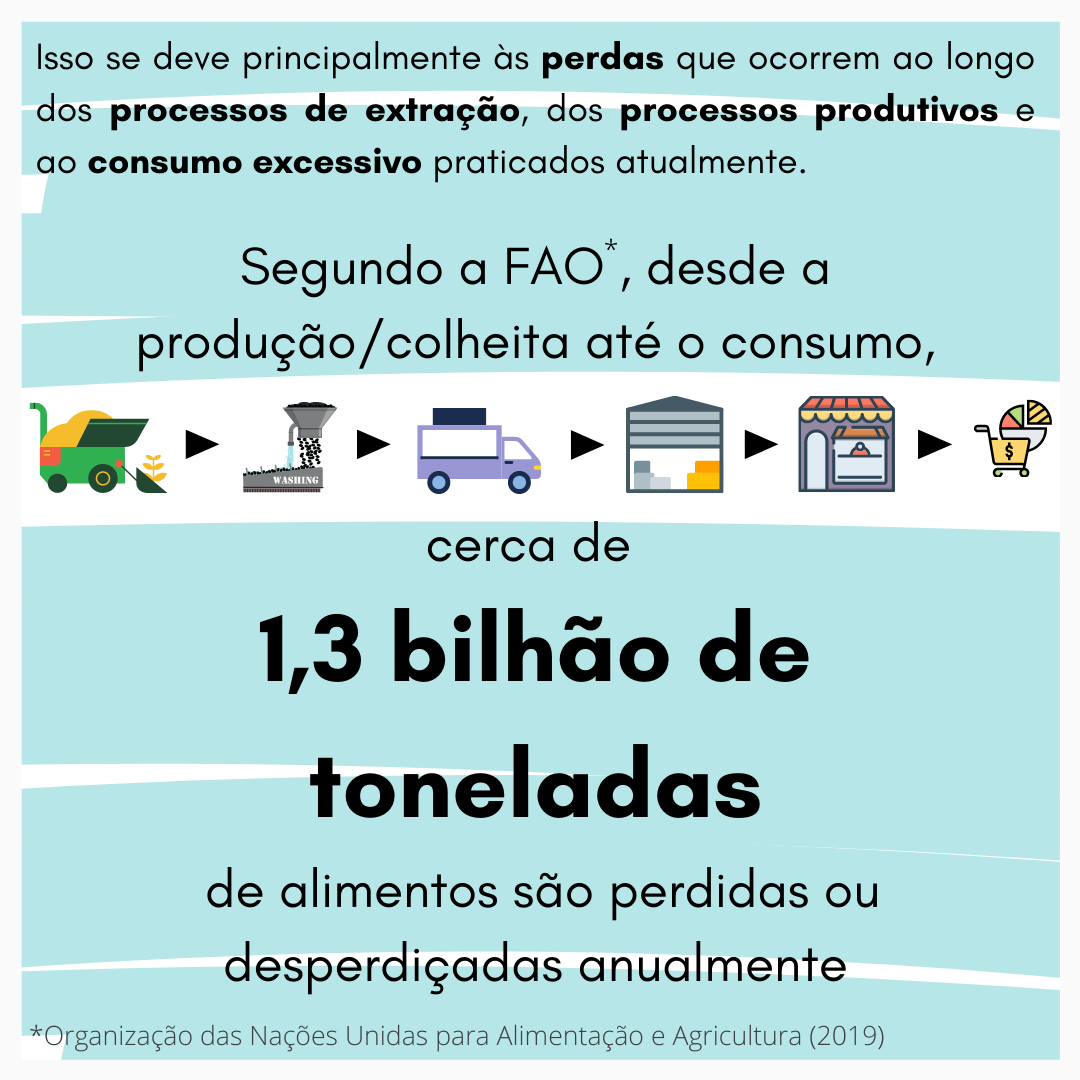
\includegraphics[width=\linewidth]{Post 3/2.png}
		\end{minipage}
	\end{frame}
	
	\begin{frame}{Post 3}
		\begin{minipage}{0.49\linewidth}
			\centering
			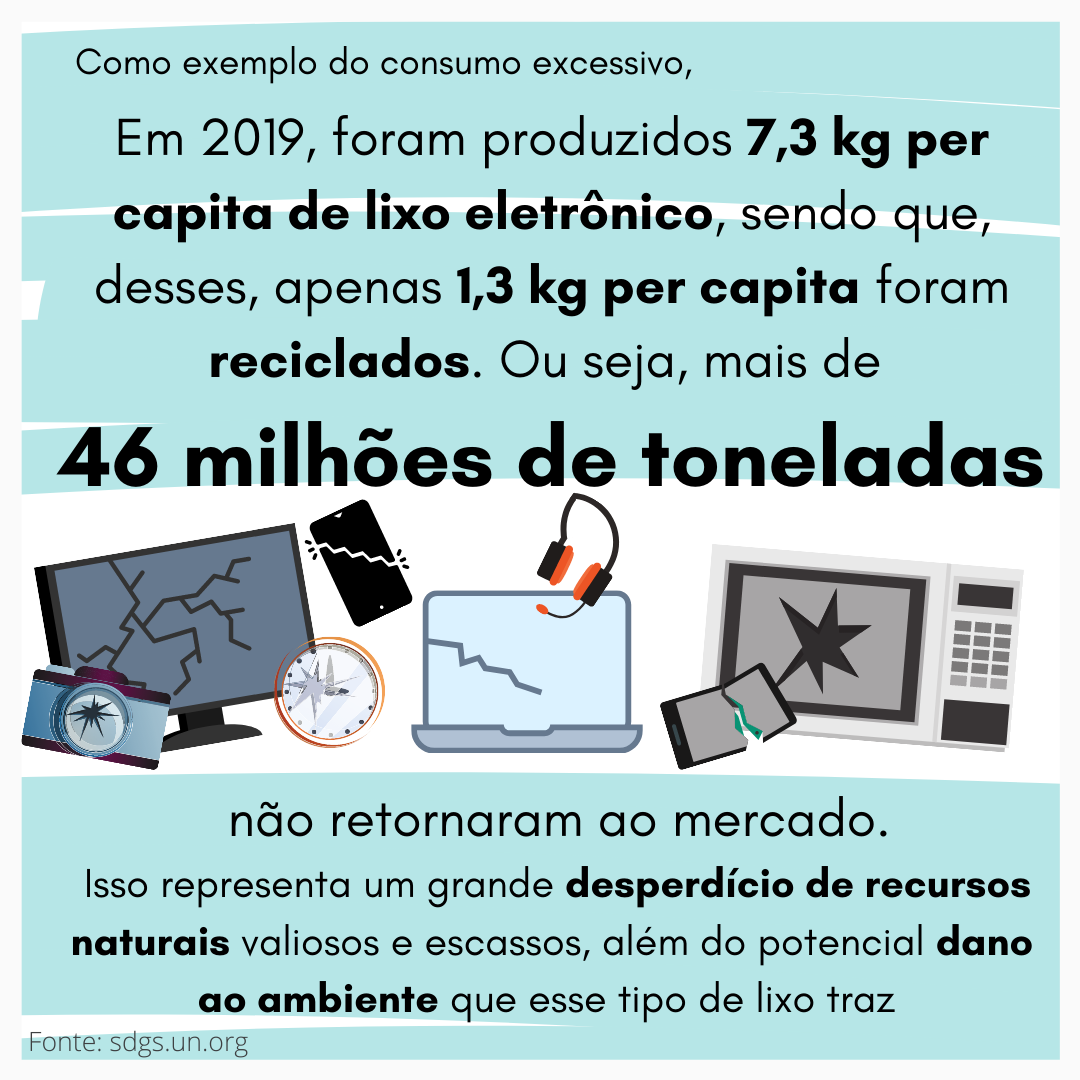
\includegraphics[width=\linewidth]{Post 3/3.png}
		\end{minipage}
		\hfill
		\begin{minipage}{0.49\linewidth}
			\centering
			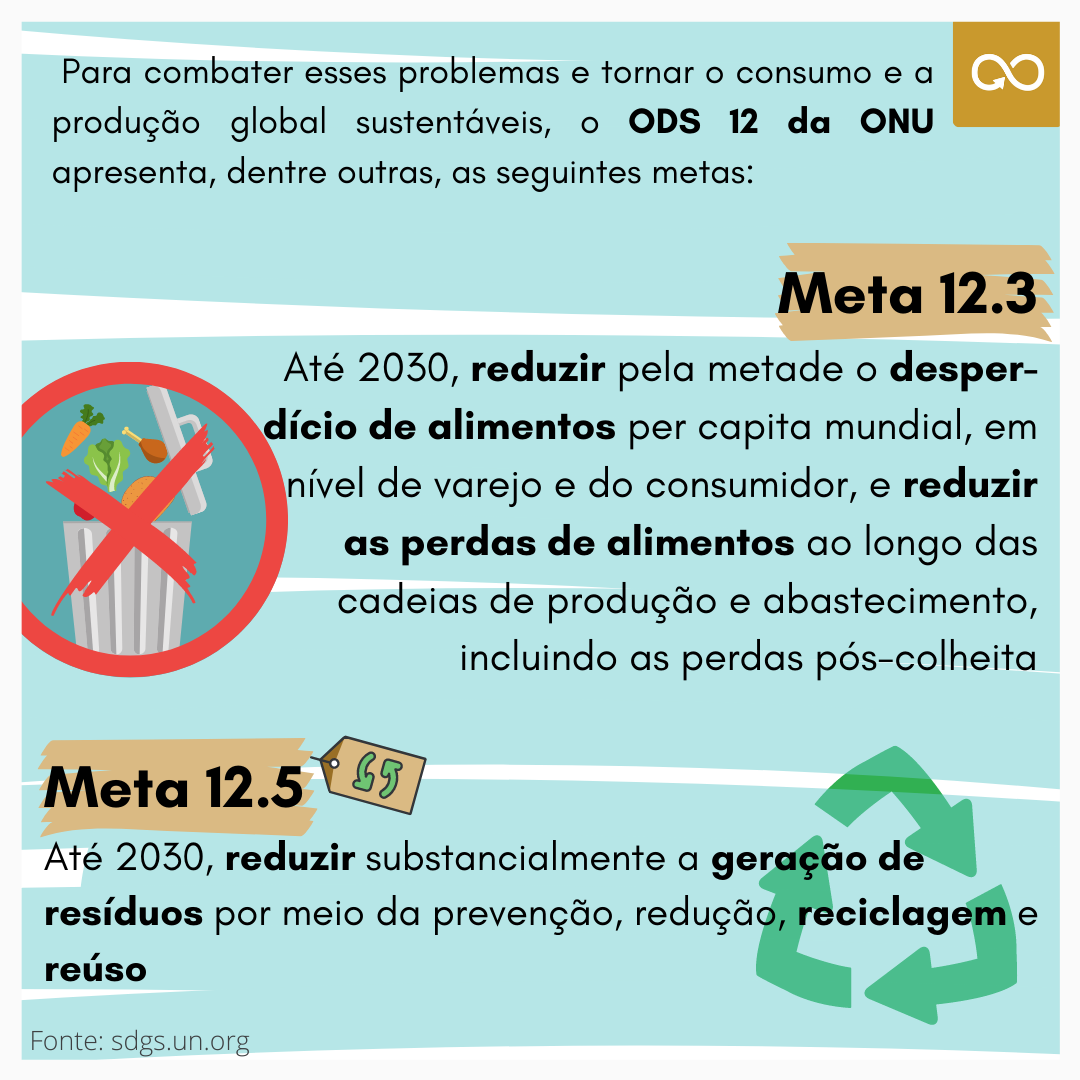
\includegraphics[width=\linewidth]{Post 3/4.png}
		\end{minipage}
	\end{frame}
	
	\begin{frame}{Post 3}
		\begin{minipage}{0.49\linewidth}
			\centering
			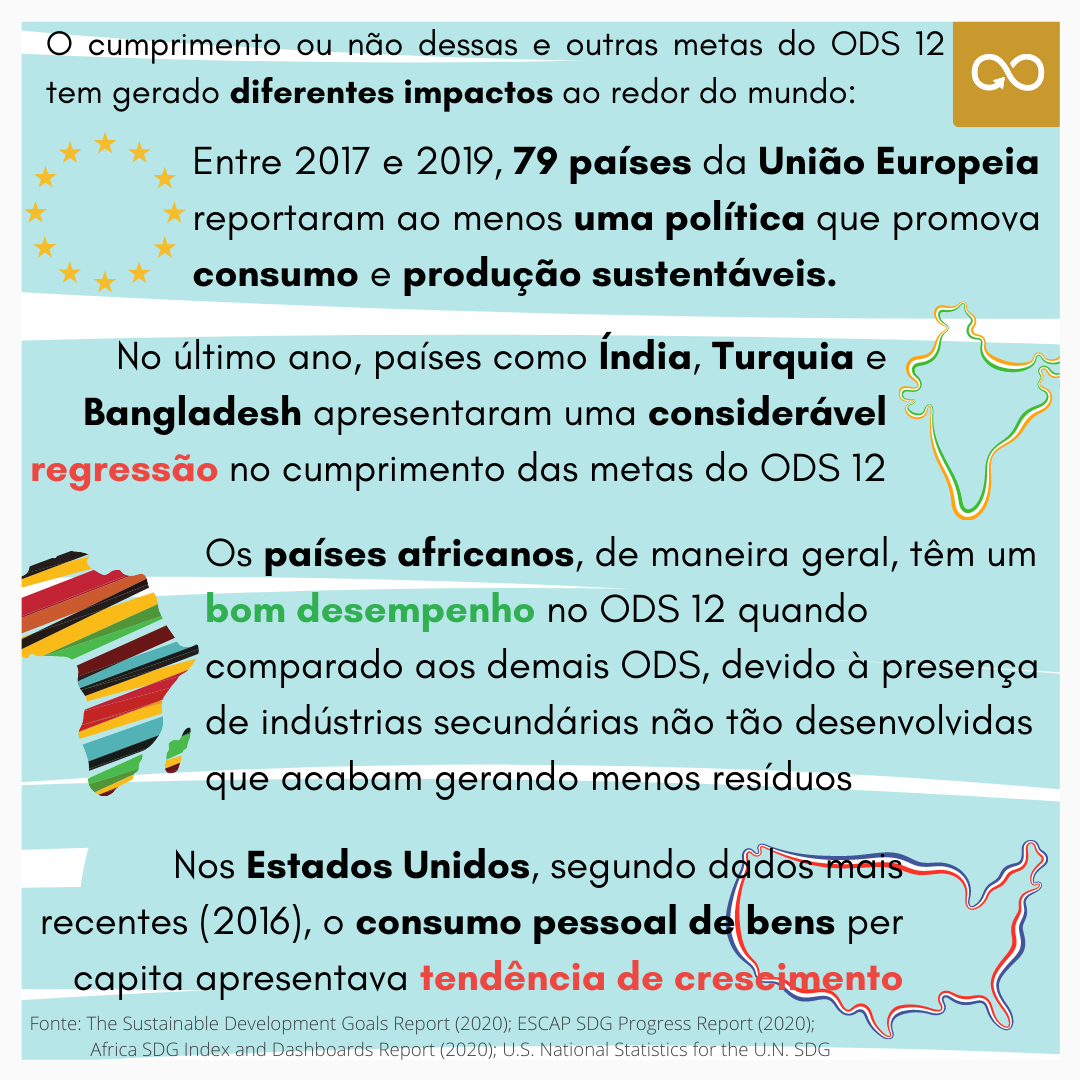
\includegraphics[width=\linewidth]{Post 3/5.png}
		\end{minipage}
		\hfill
		\begin{minipage}{0.49\linewidth}
			\centering
			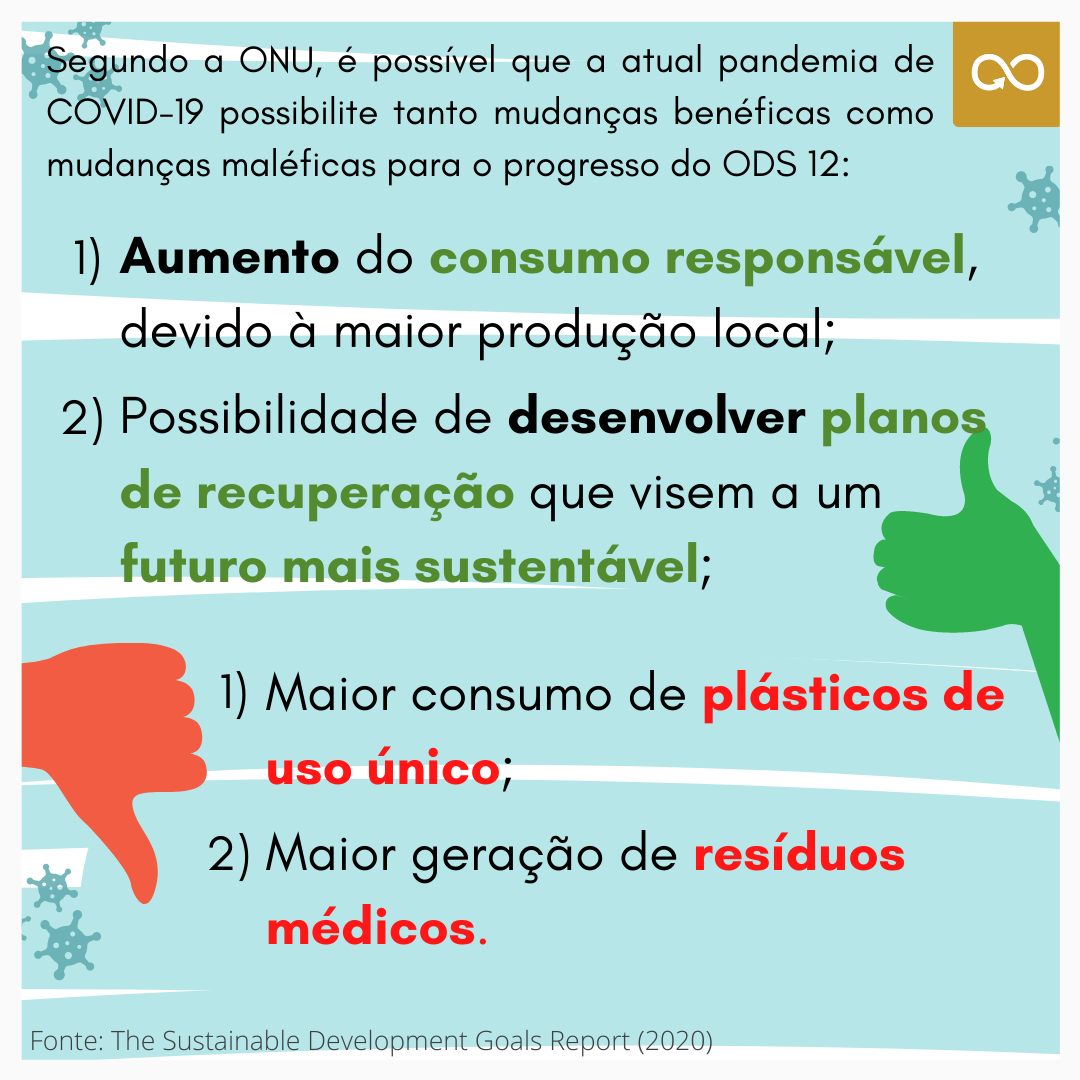
\includegraphics[width=\linewidth]{Post 3/6.png}
		\end{minipage}
	\end{frame}
	
	\begin{frame}{Post 3}
		\centering
		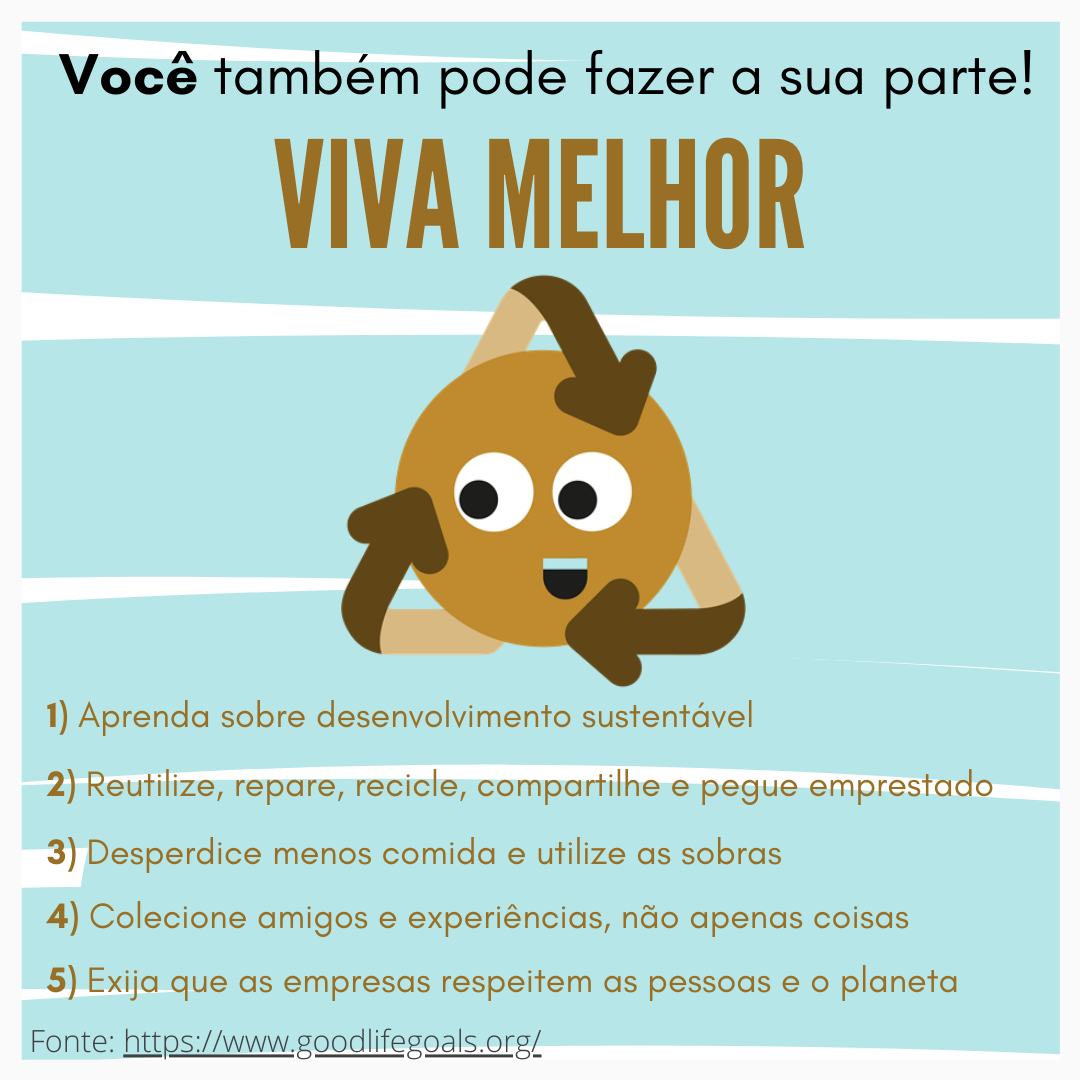
\includegraphics[width=0.7\linewidth]{Post 3/7.png}
	\end{frame}

	\begin{frame}{Página da Wikipédia}
		\begin{itemize}
			\item Traduzir $ \times $ adicionar conteúdo.
			\item Atualização de referências no novo idioma.
			\item Correção de siglas, termos e jargão.
			\item Progresso do Brasil no tema.
		\end{itemize}
	\end{frame}

	\section{Posts da Isabella --- Relatório do Ministério do Meio Ambiente}

	\begin{frame}{Acesso à informação}
		\begin{itemize}
			\item Contato para imprensa.
			\item Contato pela ouvidoria (FalaBR).
			\item Pedido por dados atualizados do progresso do Brasil na frente da ODS 12.
		\end{itemize}
	\end{frame}

	\begin{frame}[allowframebreaks]{Relatório sobre a ODS 12}
		\par\textbf{Secretaria de Qualidade Ambiental (Departamento de Gestão de Resíduos e Qualidade do Solo - DRQS, do Ministério do Meio Ambiente - MMA)}
		
		Dentre os Objetivos de Desenvolvimento Sustentável (ODS), há o Objetivo 12 que se refere ao Consumo e Produção Responsáveis. No MMA, as ações que se ajustam com o gerenciamento do uso dos recursos naturais e a forma de descarte de resíduos, estão ancoradas em importantes metas em políticas públicas que induzem a redução do desperdício, a reutilização e a reciclagem.
		
		Estão entre os objetivos da Política Nacional de Resíduos Sólidos (PNRS), coordenada pelo MMA, a não geração, redução, reutilização, reciclagem e tratamento dos resíduos sólidos, bem como disposição final ambientalmente adequada dos rejeitos. Neste contexto, o MMA tem contribuído para o ODS-12 no fortalecimento dos instrumentos de implementação da PNRS, a exemplo da publicação da proposta do Plano Nacional de Resíduos Sólidos (Planares) e, para o seu monitoramento, o Sistema Nacional de Informações sobre a Gestão dos Resíduos Sólidos (Sinir).
		
		O Planares está alinhado com o rol de programas já lançados pelo MMA entre 2019 e 2020. Como um dos principais desafios da gestão ambiental contemporânea lançou o Programa Lixão Zero e o Programa Nacional de Combate ao Lixo no Mar. As 10 metas do Planares no tema Resíduos Sólidos Urbanos estão acompanhadas de um conjunto de diretrizes e estratégias, e para o seu monitoramento no horizonte de planejamento de 20 anos (até 2040), um rol de indicadores. Algumas destas metas são:
		
		\begin{itemize}
			\item META 3: Eliminar práticas de disposição final inadequada e encerrar lixões e aterros controlados;
			\item META 4: Reduzir a quantidade de resíduos e rejeitos encaminhados para disposição final ambientalmente adequada;
			\item META 6: Aumentar a reciclagem da fração seca dos RSU;
			\item META 7: Aumentar a reciclagem da fração orgânica dos RSU.
		\end{itemize}
		
		Diante do exposto o MMA tem metas que convergem com a meta 12.5 do ODS-12 que é reduzir a geração de resíduos por meio da prevenção, redução, reciclagem e reuso, até o ano de 2030, e com a meta 12.4 que versa sobre o manejo ambientalmente adequado dos resíduos.
		
		Secretaria de Clima e Relações Internacionais:
		
		Os padrões de consumo e produção sustentáveis ​(PCS) são um tema transversal na Agenda 2030, reconhecendo seu papel facilitador na integração equilibrada de prioridades ambientais, sociais e econômicas. Todas as metas do ODS 12 têm uma associação direta  com as questões ambientais.
		
		As principais áreas são: padrões de consumo e produção sustentáveis ​(metas 12.1 e 12.2); desperdício de alimentos (12.3); produtos químicos e resíduos perigosos (12.4); prevenção, redução, reciclagem e reutilização de resíduos (12.5); compromisso corporativo (12.6); compras públicas sustentáveis ​e educação do cidadão (12.7 e 12.8); e subsídios aos combustíveis fósseis (12.c); e o turismo sustentável (12.b).
		
		O Departamento de Relações Internacionais tem como uma das suas principais atribuições promover e defender em nível internacional as políticas e os programas ambientais nacionais, em articulações bilaterais, multilaterais, regionais e globais, em coordenação com entidades governamentais e demais entidades internacionais e nacionais. Nessa perspectiva, na esfera internacional relacionada aos ODS 12, o DRI atua, entre outros, nos seguintes acordos internacionais:
		
		\begin{itemize}
			\item Convenção-Quadro das Nações Unidas sobre Mudança do Clima; Convenção sobre Diversidade Biológica;
			\item Convenção da Basiléia sobre o Controle de Movimentos Transfronteiriços de Resíduos Perigosos e sua Eliminação;
			\item Convenção de Minamata sobre Mercúrio;
			\item O Protocolo de Montreal sobre substâncias que destroem a camada de ozônio;
			\item Convenção de Rotterdam para a Aplicação do Procedimento de Consentimento Prévio Informado para Certos Produtos Químicos e Pesticidas Perigosos no Comércio Internacional;
			\item Abordagem Estratégica para Gestão Internacional de Produtos Químicos (SAICM);
			\item e Convenção de Estocolmo sobre Poluentes Orgânicos Persistentes (POPs).	
		\end{itemize}
		
		Em âmbito nacional, o Ministério do Meio Ambiente, por meio de suas áreas técnicas, implementa uma série de políticas públicas e iniciativas que contribuem para o alcance das metas do ODS 12, como algumas elencadas abaixo:
		
		\begin{itemize}
			\item O Brasil segue avançando na gestão de resíduos sólidos por meio da implantação da Política Nacional de Resíduos Sólidos, lançada em 2010. Continuam a ser implementados e ampliados acordos setoriais para aumento da logística reversa, afetando áreas como medicamentos, lâmpadas, eletrodomésticos, eletrônicos, material de embalagem, óleos lubrificantes e outros. O país também conta com o “Sistema Nacional de Informação de Resíduos Sólidos”, que está em desenvolvimento e melhoria contínua, promovendo uma gestão ambiental ampla.
			\item Como exemplo prático de política ambiental de sucesso, o Programa Lixão Zero visa eliminar lixões a céu aberto existentes no país, fortalecer a gestão integrada de resíduos sólidos, coleta seletiva, reciclagem, logística reversa, valorização energética e destinação ambientalmente adequada de resíduos. O investimento em pontos de coleta e subsequente tratamento de resíduos tem sido incentivado.
			\item No âmbito deste programa, foi recentemente assinado o ``Termo de Compromisso de Latas de Alumínio para Bebidas" entre o Ministério do Meio Ambiente e a Associação Brasileira dos Fabricantes de Latas de Alumínio (Abal) e a Associação Brasileira dos Fabricantes de Latas de Alumínio (Abralatas). A ação traz novos desafios para o setor e reforça o sucesso da reciclagem desse material no Brasil, com a inauguração de um novo centro de coleta e reciclagem em Brasília.
			\item O modelo de economia circular promovido pelo programa Lixão Zero reduz a emissão de gases com efeito de estufa e o consumo de energia do setor em mais de 70\%. O ciclo da lata envolve cerca de 800 mil pessoas, gerando renda de mais de US\$ 1 bilhão por ano.
			\item Outro exemplo é o Plano de Ação de combate ao Lixo no Mar, que tem a missão de valorizar os ambientes costeiros do país, com foco na saúde e qualidade de vida, no aumento da atratividade de praias e rios, na melhoria da qualidade do pescado, na dinamização do ecoturismo, na geração de emprego e renda, no fortalecimento das cadeias de reciclagem e na conservação da vida marinha.
			\item Sob a agenda de promoção de ecoturismo, o Ministério do Meio Ambiente vem desenvolvendo ações de estímulo ao turismo nos parques nacionais, como São Joaquim, Descobrimento e Ubajara abriram editais para guias turísticos. Costa dos Corais e Abrolhos tiveram editais para transporte aquaviário, enquanto as florestas nacionais de Ipanema e de Brasília abriram editais para comércio de alimentos para os visitantes. A importância dessas ações vai além dos empregos diretos, gerados dentro dos parques, e dos empregos indiretos, gerados ao longo de toda a cadeia do ecoturismo, dinamizada pelo aumento da visitação. O aquecimento do setor contribui, principalmente, para a proteção ambiental, envolvendo as comunidades da região na conservação dos parques.
			\item A Agenda Ambiental da Administração Pública (A3P) é um Programa do MMA, que por meio dos seus eixos de trabalho busca criar uma cultura de responsabilidade socioambiental na administração pública e, para tanto, estrutura-se em seis Eixos Temáticos prioritários fundamentados pela política dos 5 R’s: Repensar, Reduzir, Reaproveitar, Reciclar e Recusar o consumo de produtos que gerem impactos socioambientais negativos significativos. (Eixos de trabalho da A3P: compras públicas sustentáveis, uso racional dos recursos naturais e bens públicos, gestão adequada dos resíduos gerados, qualidade de vida no ambiente de trabalho, construções sustentáveis e sensibilização e capacitação dos servidores).	
		\end{itemize}

	\end{frame}

	\begin{frame}{Post 4}
		\begin{minipage}{0.49\linewidth}
			\centering
			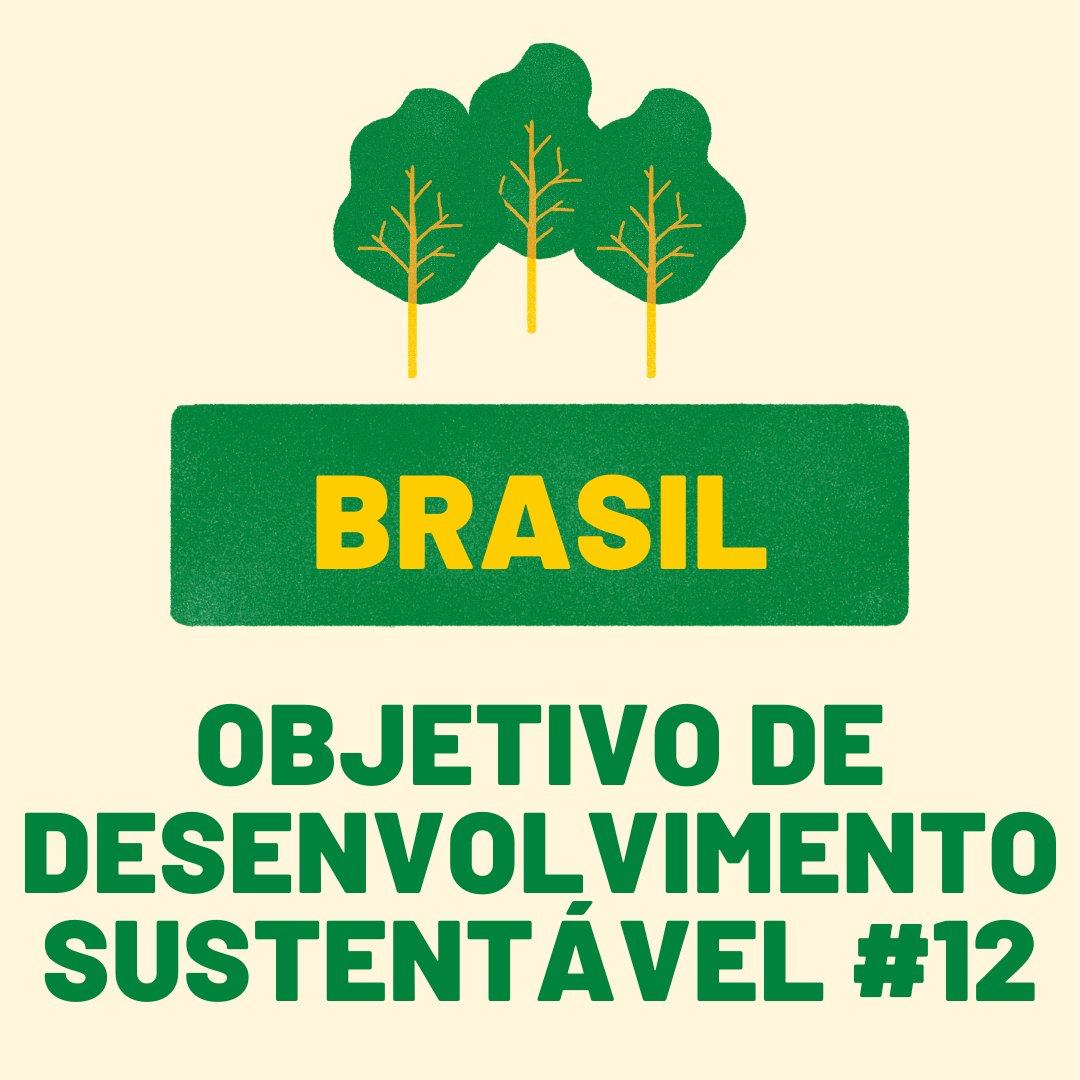
\includegraphics[width=\linewidth]{Post 4/1.png}
		\end{minipage}
		\hfill
		\begin{minipage}{0.49\linewidth}
			\centering
			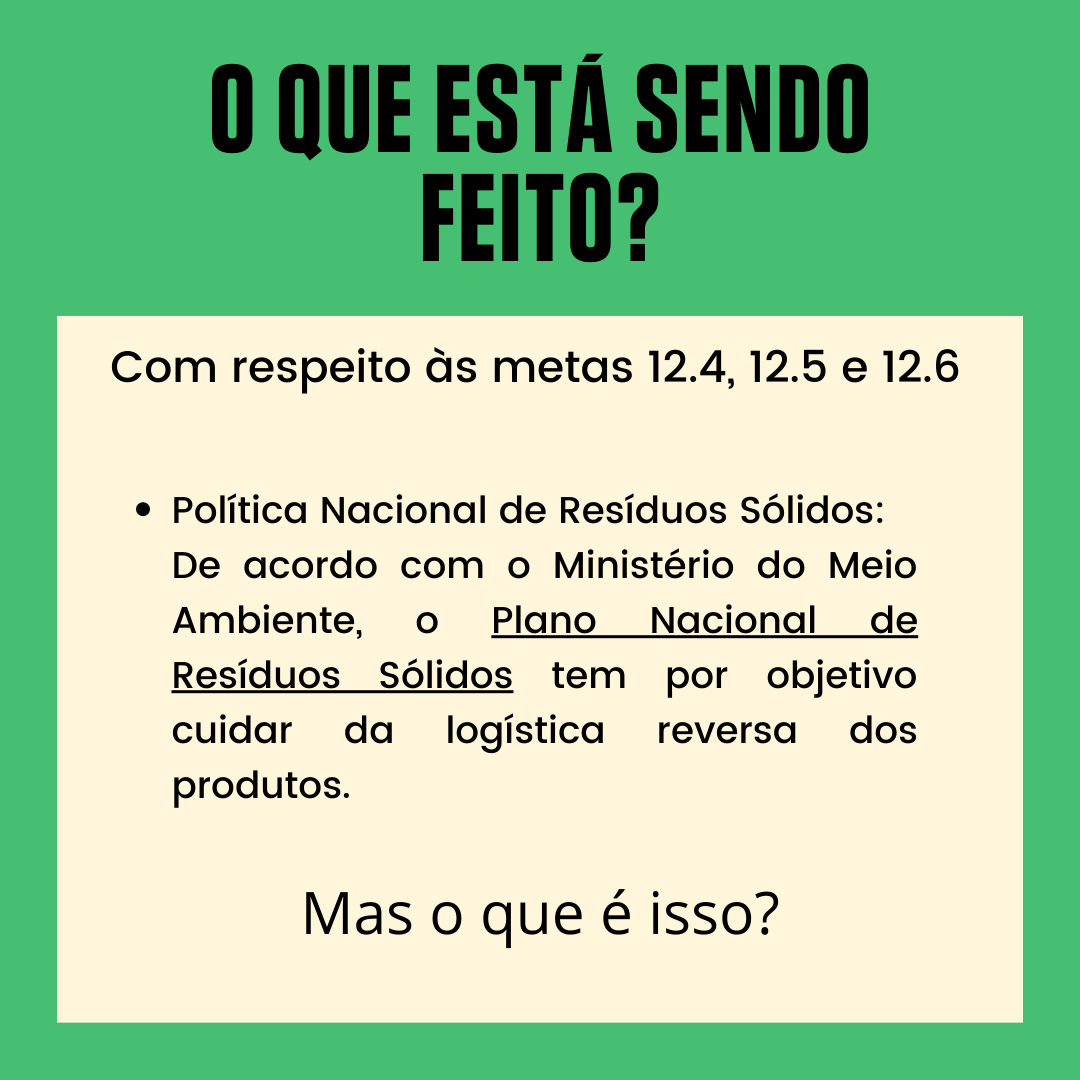
\includegraphics[width=\linewidth]{Post 4/2.png}
		\end{minipage}
	\end{frame}
	
	\begin{frame}{Post 4}
		\begin{minipage}{0.49\linewidth}
			\centering
			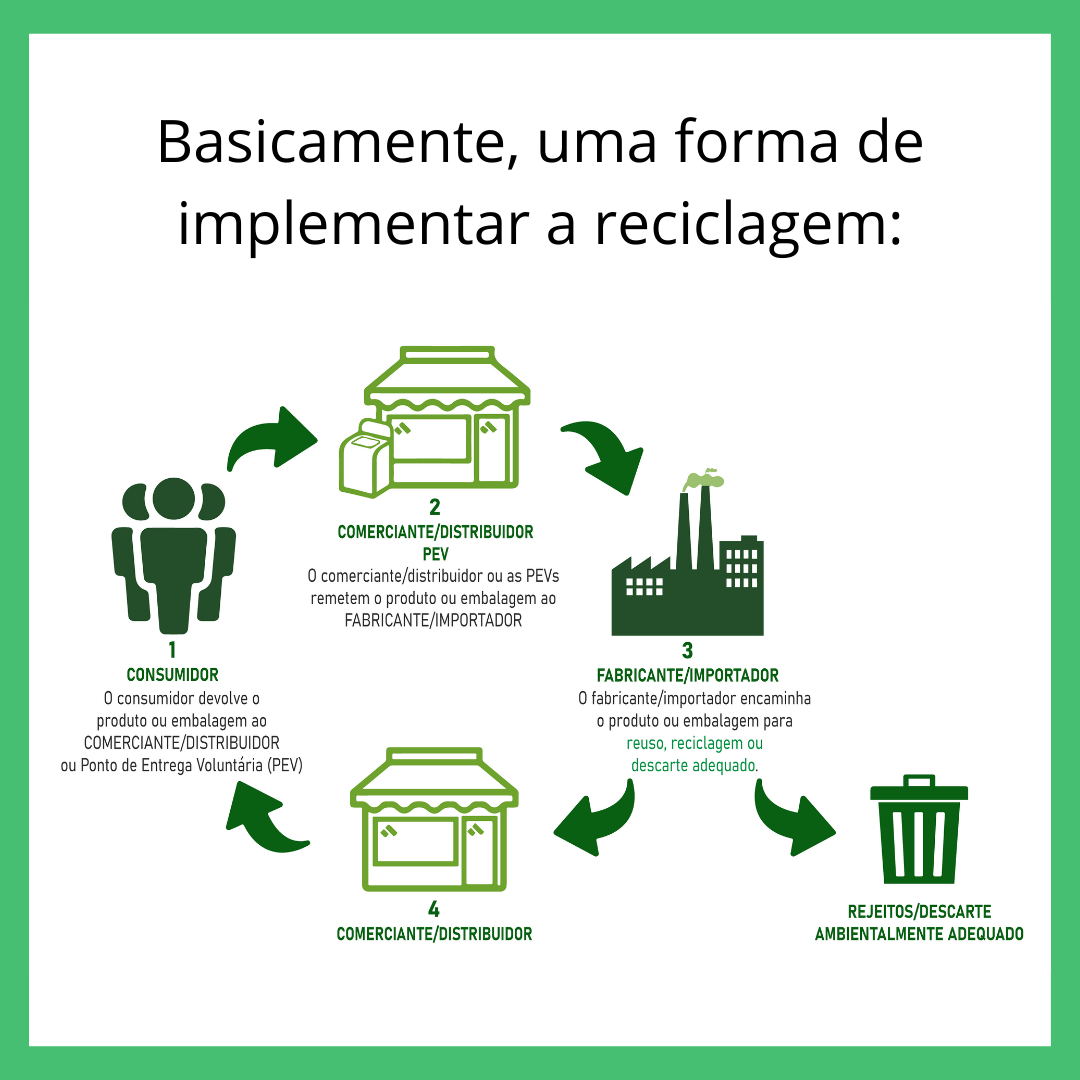
\includegraphics[width=\linewidth]{Post 4/3.png}
		\end{minipage}
		\hfill
		\begin{minipage}{0.49\linewidth}
			\centering
			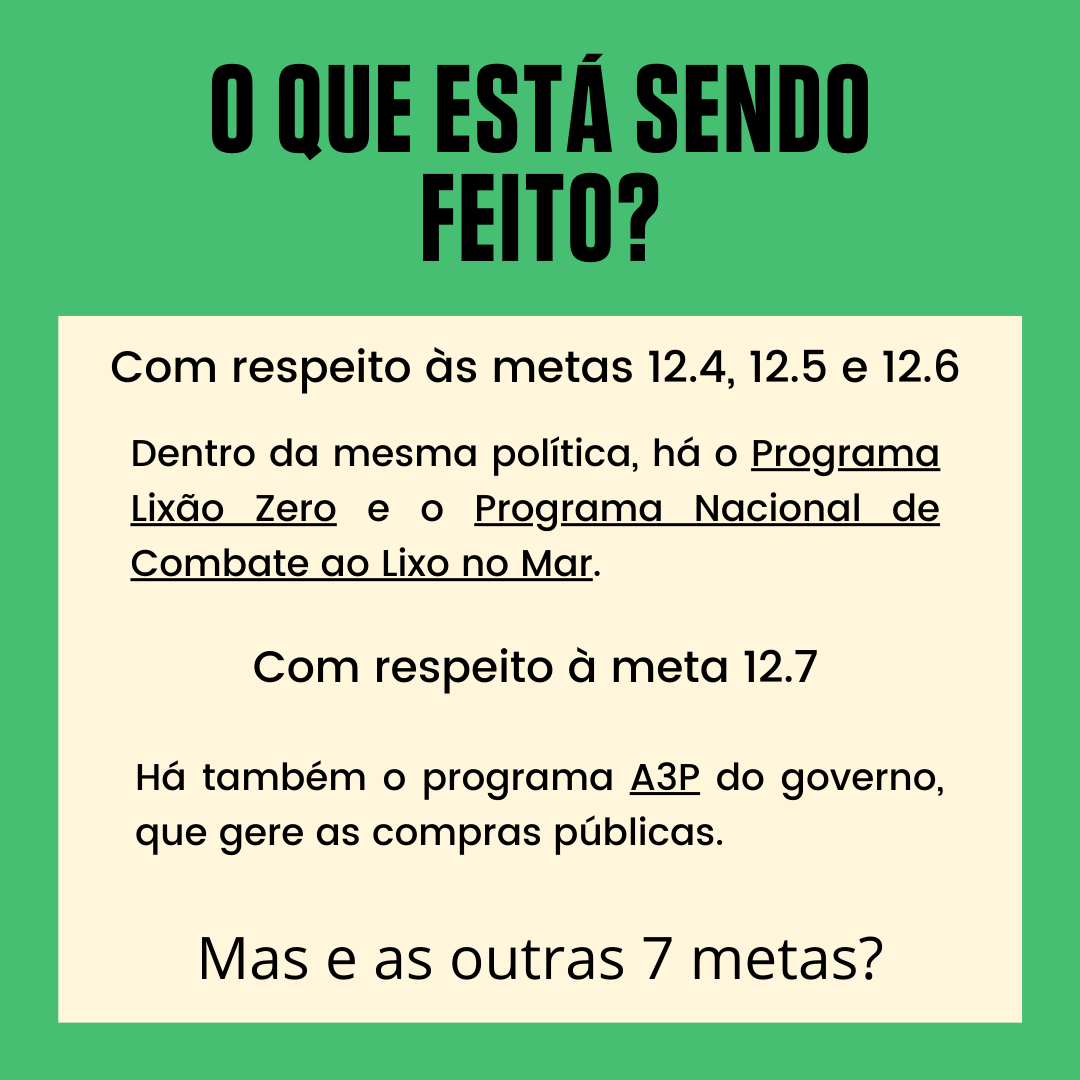
\includegraphics[width=\linewidth]{Post 4/4.png}
		\end{minipage}
	\end{frame}
	
	\begin{frame}{Post 4}
		\begin{minipage}{0.49\linewidth}
			\centering
			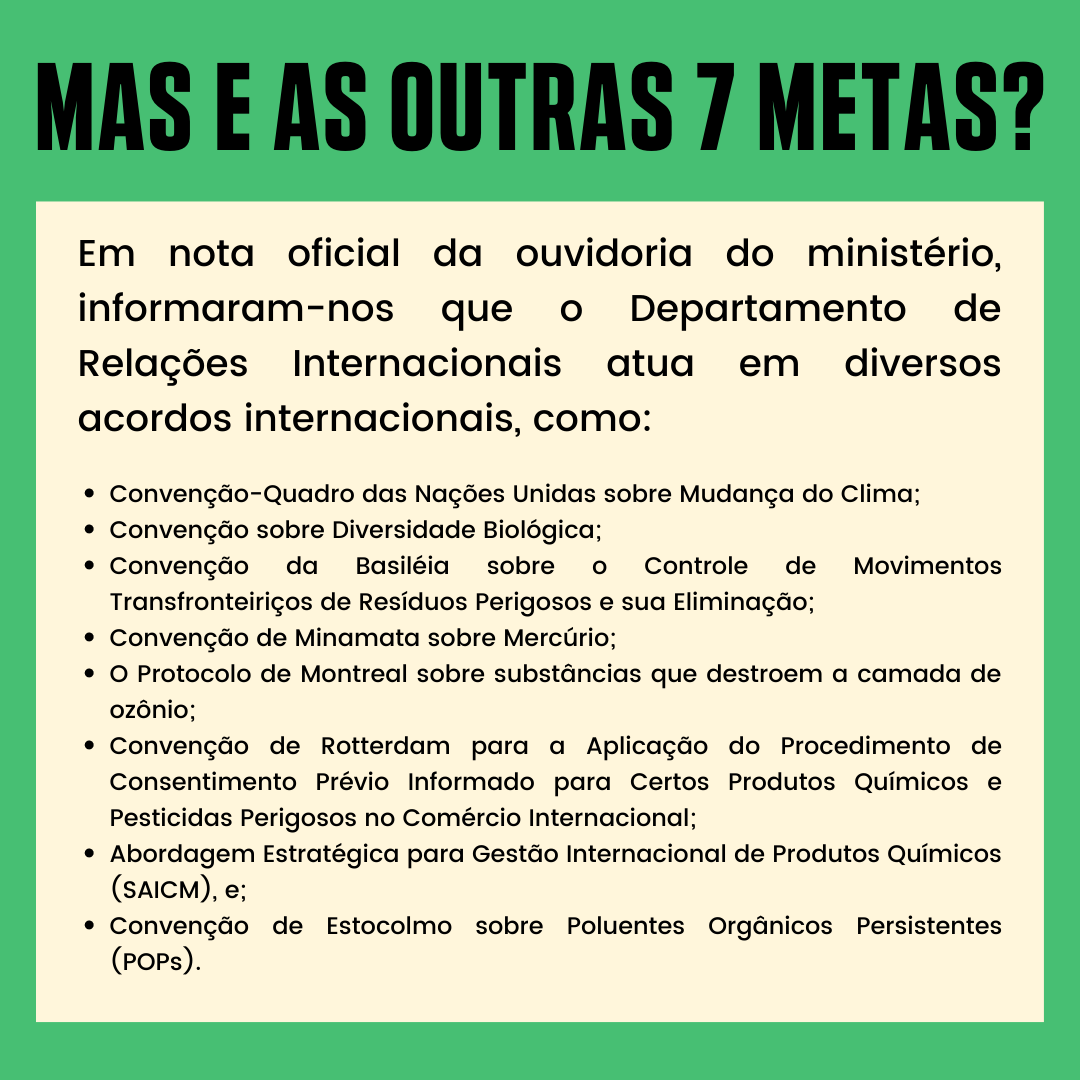
\includegraphics[width=\linewidth]{Post 4/5.png}
		\end{minipage}
		\hfill
		\begin{minipage}{0.49\linewidth}
			\centering
			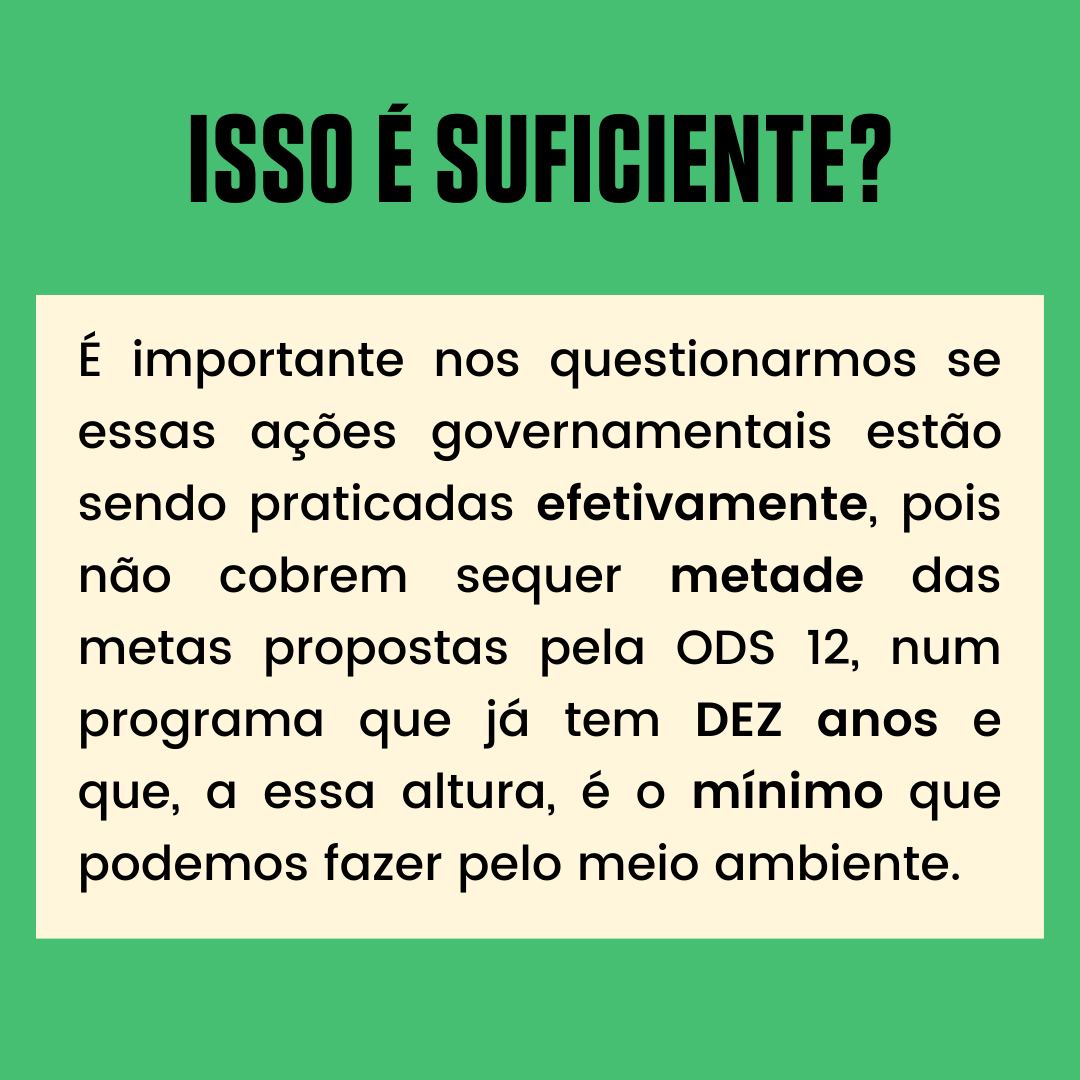
\includegraphics[width=\linewidth]{Post 4/6.png}
		\end{minipage}
	\end{frame}

\end{document}